\documentclass[12pt,a4paper,spanish]{article} 
\usepackage{babel}
\usepackage [T1]{fontenc}
\usepackage [latin1]{inputenc}
\usepackage{graphicx} 
\usepackage{float}
\usepackage{verbatim}
\usepackage{array}
	  \oddsidemargin 0in
      \textwidth 6.75in
      \topmargin 0in
      \textheight 10.0in
      \parindent 0em
      \parskip 2ex
\usepackage{anysize}
\marginsize{3cm}{2cm}{1.0cm}{1.0cm}

\usepackage{moreverb}





\pagestyle{plain}

\begin{document} 
\title{
\begin{table}[!h]
	\begin{tabular}{m{2cm}m{15cm}}
		\multicolumn{1}{l}{} &
		 
\includegraphics[scale=0.5, bb=0 0 0 0]{../logo-fiuba.PNG} & 
		 \begin{center}
		 	\begin{LARGE}
				Universidad de Buenos Aires	\linebreak \linebreak		 							Facultad de Ingenier\'{i}a  \linebreak \linebreak
				7515 - Base de Datos \linebreak \linebreak
				1er. Cuatrimestre de 2010
			\end{LARGE}
		 \end{center}\\
\end{tabular}
\end{table}
\begin{Large}
 \begin{center}
		\underline{TP Base de Datos: SIGeek} \linebreak \linebreak
        Docente a cargo: Ing. Lucas Roman
\end{center}
\end{Large}
}
\date{}
\maketitle

\thispagestyle{empty}
\author{
\begin{Large}
\begin{center}
		\underline{Integrantes}  \linebreak 
\end{center}
\end{Large}
\begin{center}
	\begin{tabular}{|| c | c | c ||}
		\hline
		\begin{large}Apellido y Nombre\end{large} & 
		\begin{large}Padr\'{o}n Nro.\end{large} & 
		\begin{large}E-mail\end{large}\\
		\hline
		Bruno Tom�s & 88.449 & tbruno88@gmail.com\\
		\hline
		Invernizzi Esteban Ignacio & 88.817 & invernizzie@gmail.com\\
		\hline
		Meller Gustavo Ariel  & 88.435 & gmeller@gmail.com\\
		\hline
		Rivero Hern\'an Javier & 88.455 & riverohernanj@gmail.com\\
		\hline
	\end{tabular}
\end{center}
}

\newpage
\setcounter{page}{1} 
\tableofcontents
\newpage

\section{Introducci�n}

	Esta segunda entrega consta de la resoluci�n y la expresi�n en lenguaje SQL de once consultas, contra un esquema relacional propuesto por la c�tedra. Las sentencias y cl�usulas a utilizar fueron restringidas a las presentadas por la c�tedra en la cartilla del apunte del lenguaje SQL.

\clearpage
\section{Consultas y resoluci�n}
	
	\subsection*{Consulta 1}
	
		 \textit{El promedio de mothers pedidas por pedido}

		\small
		\begin{verbatimtab}

SELECT sum(CANT_PEDIDA) / (count(distinct PEDIDO.NRO_PEDIDO) 
				* count(distinct PEDIDO.NRO_PEDIDO)) PROMEDIO
FROM PEDIDO, ITEM_PEDIDO, SUBTIPO_COMPONENTE
WHERE 	ITEM_PEDIDO.SUBTIPO = SUBTIPO_COMPONENTE.SUBTIPO
		AND TIPO = 'MOTHER'

  		\end{verbatimtab}
		\normalsize

		Hip�tesis: Hay alg�n pedido de mothers.		

		\small
		\begin{verbatimtab}		

SELECT sum(CANT_PEDIDA) / count(DISTINCT NRO_PEDIDO) PROMEDIO
FROM (	
	SELECT NRO_PEDIDO, SUBTIPO, CANT_PEDIDA
	FROM ITEM_PEDIDO
	UNION
	SELECT NRO_PEDIDO, I.SUBTIPO, -CANT_PEDIDA
	FROM ITEM_PEDIDO I, SUBTIPO_COMPONENTE S
	WHERE I.SUBTIPO = S.SUBTIPO AND TIPO <> 'MOTHER' )
					
		\end{verbatimtab}
		\normalsize
		
		
			\begin{figure}[H]
			\centering
			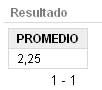
\includegraphics[scale=1]{resultados/1.jpg}
			\end{figure}

	\clearpage
	\subsection*{Consulta 2}
	\textit{La raz�n social de los proveedores tales que existe un producto
que no comercializan.}
	
			\small
			
			\begin{verbatimtab}

SELECT RAZON_SOCIAL
FROM PROVEEDOR pr1
WHERE EXISTS (	
	SELECT * 
	FROM TIPO_COMPONENTE
	WHERE NOT EXISTS(
		SELECT * 
		FROM CATALOGO_PROVEEDOR, SUBTIPO_COMPONENTE
		WHERE CATALOGO_PROVEEDOR.SUBTIPO = SUBTIPO_COMPONENTE.SUBTIPO
		AND pr1.CUIT = CATALOGO_PROVEEDOR.CUIT
		AND SUBTIPO_COMPONENTE.TIPO = TIPO_COMPONENTE.TIPO))
		
		\end{verbatimtab}
		\normalsize
		
		   
			\begin{figure}[H]
			\centering
			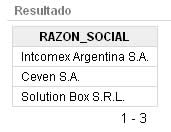
\includegraphics[scale=1]{resultados/2.jpg}
			\end{figure}		
		
		\clearpage
		\subsection*{Consulta 3}
		\textit{Un listado alfab�tico de subtipos de componentes a reponer indicando tipo de componente, subtipo de componente y razon$\_$social de los proveedores que los comercializan.}
		
		\small
		\begin{verbatimtab}
	
SELECT TIPO,  S.SUBTIPO, RAZON_SOCIAL
FROM SUBTIPO_COMPONENTE S, CATALOGO_PROVEEDOR C, PROVEEDOR P
WHERE 	S.SUBTIPO = C.SUBTIPO 
		AND C.CUIT = P. CUIT 
		AND CANT_STOCK < CANT_MINIMA
ORDER BY TIPO, SUBTIPO

		\end{verbatimtab}
		\normalsize
		
		

			\begin{figure}[H]
			\centering
			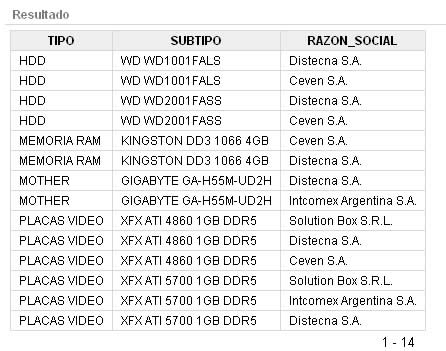
\includegraphics[scale=0.75]{resultados/3.jpg}
			\end{figure}	
		
		\clearpage
		\subsection*{Consulta 4}
		\textit{La razon$\_$social de los proveedores que comercializan todos los subtipos de componentes a reponer.}
		
		\small
		\begin{verbatimtab}
			
SELECT RAZON_SOCIAL
FROM PROVEEDOR P
WHERE NOT EXISTS (
	SELECT 'SUBTIPO A REPONER NO COMECIALIZADO'
	FROM SUBTIPO_COMPONENTE S	
	WHERE CANT_STOCK < CANT_MINIMA 
	AND NOT EXISTS(
		SELECT 'SUBTIPO EN CATALOGO'
		FROM CATALOGO_PROVEEDOR C
		WHERE P.CUIT = C.CUIT AND S.SUBTIPO = C.SUBTIPO))

		\end{verbatimtab}
		\normalsize
			
		  
			\begin{figure}[H]
			\centering
			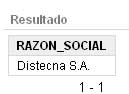
\includegraphics[scale=1]{resultados/4.jpg}
			\end{figure}		
		
		\clearpage
		\subsection*{Consulta 5}
		\textit{La razon$\_$social, el nro$\_$pedido y el subtipo de componente de los �tems de pedidos de subtipos de componente no comercializados por el proveedor del pedido.}
		
		Interpretaci�n: Obtener los pedidos a proveedores que contienen un item pedido que ese proveedor no comercializa.
		
		\small
		\begin{verbatimtab}
		
SELECT RAZON_SOCIAL, PE.NRO_PEDIDO, SUBTIPO
FROM PROVEEDOR PR, PEDIDO PE, ITEM_PEDIDO I
WHERE 	PR.CUIT = PE.CUIT 
		AND PE.NRO_PEDIDO = I.NRO_PEDIDO
		AND I.SUBTIPO NOT IN (
			SELECT SUBTIPO
			FROM CATALOGO_PROVEEDOR C
			WHERE C.CUIT = PR. CUIT) 

		\end{verbatimtab}
		\normalsize
		
		
			\begin{figure}[H]
			\centering
			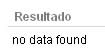
\includegraphics[scale=1]{resultados/5.jpg}
			\end{figure}		
		
		\clearpage
		\subsection*{Consulta 6}
		\textit{La razon$\_$social de los proveedores que comercializan exclusivamente un tipo de componente.}
		
		\subsubsection*{Interpretaci�n 1}
			La raz�n social de los proveedores que proveen un solo tipo de componente.
		
		\small
		\begin{verbatimtab}
SELECT DISTINCT RAZON_SOCIAL
FROM PROVEEDOR P, CATALOGO_PROVEEDOR C1, SUBTIPO_COMPONENTE S1
WHERE P.CUIT = C1.CUIT  
AND S1.SUBTIPO = C1.SUBTIPO
AND NOT EXISTS (
	SELECT 'OTRO TIPO PROVISTO'
	FROM CATALOGO_PROVEEDOR C2, SUBTIPO_COMPONENTE S2
	WHERE C2.SUBTIPO = S2.SUBTIPO 
	AND C1.CUIT = C2.CUIT 
	AND S1.TIPO <> S2.TIPO)
		\end{verbatimtab}
		\normalsize

			\begin{figure}[H]
			\centering
			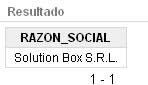
\includegraphics[scale=1]{resultados/6a.jpg}
			\end{figure}	
			
		\subsubsection*{Interpretaci�n 2}
		La raz�n social de los proveedores que tienen en su catalogo un tipo de componente que no esta en el catalogo de ning�n otro proveedor.
		
		\small
		\begin{verbatimtab}	
SELECT P.RAZON_SOCIAL
FROM PROVEEDOR P, CATALOGO_PROVEEDOR CP, SUBTIPO_COMPONENTE S
WHERE P.CUIT = CP.CUIT
AND CP.SUBTIPO = S.SUBTIPO
AND NOT EXISTS (
	SELECT *
	FROM PROVEEDOR P2, CATALOGO_PROVEEDOR CP2, SUBTIPO_COMPONENTE S2
	WHERE P2.CUIT = CP2.CUIT
	AND CP2.SUBTIPO = S2.SUBTIPO
	AND P.CUIT <> P2.CUIT
	AND S.TIPO = S2.TIPO )
		\end{verbatimtab}
		\normalsize

			\begin{figure}[H]
			\centering
			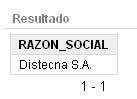
\includegraphics[scale=1]{resultados/6b.jpg}
			\end{figure}		
			
		\clearpage
		\subsection*{Consulta 7}
		\textit{El subtipo de los componentes entregados exclusivamente por el proveedor 'Ceven S.A.'.}
		
		Hip�tesis: Los items entregados son los que se encuentran en ITEM$\_$PEDIDO con CANT$\_$RECIBIDA mayor a cero.
		
		\small
		\begin{verbatimtab}		
		
SELECT SUBTIPO
FROM SUBTIPO_COMPONENTE S
WHERE EXISTS (
	SELECT 'ENTREGA DE CEVEN S.A.'
	FROM ITEM_PEDIDO I1, PEDIDO PE1, PROVEEDOR PR1
	WHERE S.SUBTIPO = I1.SUBTIPO 
	AND PE1.NRO_PEDIDO = I1.NRO_PEDIDO 
	AND PR1.CUIT = PE1.CUIT
	AND CANT_RECIBIDA > 0 
	AND RAZON_SOCIAL = 'Ceven S.A.' )
AND NOT EXISTS (
	SELECT 'ENTREGA DE CEVEN S.A.'
	FROM ITEM_PEDIDO I2, PEDIDO PE2, PROVEEDOR PR2
	WHERE S.SUBTIPO = I2.SUBTIPO 
	AND PE2.NRO_PEDIDO = I2.NRO_PEDIDO 
	AND PR2.CUIT = PE2.CUIT
	AND CANT_RECIBIDA > 0 
	AND RAZON_SOCIAL <> 'Ceven S.A.' )
					
		\end{verbatimtab}
		\normalsize

		
			\begin{figure}[H]
			\centering
			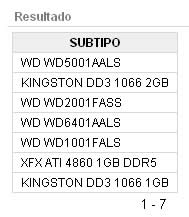
\includegraphics[scale=1]{resultados/7.jpg}
			\end{figure}		
		
		\clearpage
		\subsection*{Consulta 8}
		\textit{El subtipo de los componentes para los cuales el stock informado es distinto del real.}
		
		Hipotesis: los componentes que existen en COMPONENTE no son utilizados en PCs y no estan reservadas para ordenes, forman parte del stock.
		
		\small
		\begin{verbatimtab}

SELECT SUB.SUBTIPO
FROM SUBTIPO_COMPONENTE SUB
WHERE SUB.CANT_STOCK <> (
	SELECT count(*)
	FROM COMPONENTE COMP
	WHERE SUB.SUBTIPO = COMP.SUBTIPO
	AND  COMP.CODIGO_PC IS NULL
	AND  COMP.NRO_ORDEN IS NULL )
						
		\end{verbatimtab}
		\normalsize
		
		
			\begin{figure}[H]
			\centering
			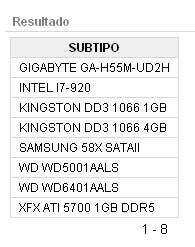
\includegraphics[scale=1]{resultados/8.jpg}
			\end{figure}		
		
		\clearpage
		\subsection*{Consulta 9}
		\textit{El nro$\_$pedido y el subtipo de componentes de los �tems de pedidos cuya cantidad pedida supere a la cantidad pedida promedio de ese subtipo de componentes.}
		
		\small
		\begin{verbatimtab}
SELECT ITEM.NRO_PEDIDO, ITEM.SUBTIPO
FROM ITEM_PEDIDO ITEM
WHERE ITEM.CANT_PEDIDA > ( SELECT avg(ITEM2.CANT_PEDIDA)
                           FROM ITEM_PEDIDO ITEM2
                           WHERE ITEM2.SUBTIPO = ITEM.SUBTIPO )			   
		
		\end{verbatimtab}
		\normalsize
		
			\begin{figure}[H]
			\centering
			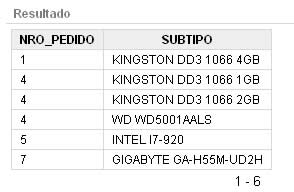
\includegraphics[scale=1]{resultados/9.jpg}
			\end{figure}		
		
		\clearpage
		\subsection*{Consulta 10}
		\textit{ Para cada tipo de componente el subtipo de componente que tenga la mayor cantidad recibida.}
		
		
		\small
		\begin{verbatimtab}
		
SELECT TIPO, S1.SUBTIPO
FROM SUBTIPO_COMPONENTE S1, ITEM_PEDIDO I1
WHERE S1.SUBTIPO = I1.SUBTIPO
GROUP BY TIPO,  S1.SUBTIPO
HAVING SUM (CANT_RECIBIDA) >= ALL (
	SELECT SUM(CANT_RECIBIDA)
	FROM  SUBTIPO_COMPONENTE S2, ITEM_PEDIDO I2
	WHERE S2.SUBTIPO = I2.SUBTIPO AND S2.TIPO = S1.TIPO
	GROUP BY S2.SUBTIPO )
ORDER BY TIPO

		\end{verbatimtab}
		\normalsize		
		
		
			\begin{figure}[H]
			\centering
			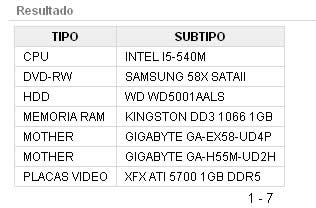
\includegraphics[scale=1]{resultados/10.jpg}
			\end{figure}		
		
		\clearpage
		\subsection*{Consulta 11}
		\textit{ El subtipo de los componentes entregados por todos los proveedores que comercializan todos los tipos de componentes.}
		
		
		
		\small
		\begin{verbatimtab}
		
SELECT SUBTIPO
FROM SUBTIPO_COMPONENTE S1
WHERE NOT EXISTS (
	SELECT 'PROVEDOR DE TODOS LOS TIPOS QUE NO LO ENTREGA'
	FROM PROVEEDOR PR
	WHERE NOT EXISTS (
		SELECT 'TIPO NO ENTREGADO'
		FROM TIPO_COMPONENTE T
		WHERE NOT EXISTS (
			SELECT 'TIPO EN CATALOGO'
			FROM SUBTIPO_COMPONENTE S2, 
				CATALOGO_PROVEEDOR C
			WHERE S2.TIPO = T.TIPO 
			AND C.CUIT = PR.CUIT 
			AND C.SUBTIPO = S2.SUBTIPO ) )
	AND PR.CUIT NOT IN (
		SELECT PE.CUIT
		FROM ITEM_PEDIDO I, PEDIDO PE
		WHERE I.NRO_PEDIDO = PE.NRO_PEDIDO 
		AND S1.SUBTIPO=I.SUBTIPO 
		AND CANT_RECIBIDA > 0 ) )

		\end{verbatimtab}
		\normalsize
		
		
			\begin{figure}[H]
			\centering
			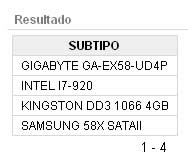
\includegraphics[scale=1]{resultados/11.jpg}
			\end{figure}		

\end{document}
